\chapter{Set-up sperimentale}

\section{Procedura di misurazione}
Le mappe di flusso stimate esprimono il flusso magnetico in funzione delle componenti di corrente d-q e la posizione meccanica.\\
L'area di valutazione del modello è  un rettangolo nel piano $dq$. Tale rettangolo deve contenere tutte i punti di interesse per l'azionamento sotto test \cite{Armando}.\\
L'area viene così organizzata in una griglia equispaziata, individuata dai vettori di corrente della griglia:
\begin{equation}
\begin{cases}
    i_{d,k} = i_{d,\min} + k \cdot \Delta i_d & k = 1, 2, 3 \\
    i_{q,k'} = i_{q,\min} + k' \cdot \Delta i_q & k' = 1, 2, 3.
\end{cases}
\end{equation}

%\subsection{Procedura di misurazione}
%Bisogna anche tenere conto %del rischio di %smagnetizzazione.

\subsection{Set-up sperimentale}
Nel set-up sperimentale il motore di test (MUT) è accoppiato da un motore controllato in velocità. Tale motore trascina il motore di test imponendo una velocità di rotazione costante, l'articolo \cite{bojoi2024} propone una velocità pari a 1/3 della velocità nominale del motore di test.\\
Tenere una velocità elevata permette di ridurre l'effetto delle perdite nel ferro e nel magnete permanente durante il test.\\
Il MUT viene controllato in corrente. I valori di corrente di riferimento sono i punti della griglia di corrente sui quali si vuole stimare il flusso.\\
Dato che cge si adotta la convenzione degli a assi PM, il dominio dell'esplorazione del flusso copre il primo e il secondo quadrante del piano $i_{dq}$. Il dominio di corrente considerato è $i_d \in [-10\,\text{A}; 10\,\text{A}]$ e $i_q \in [0\,\text{A}; 10\,\text{A}]$.\\
Con riferimento al generico $k$-esimo punto di corrente $i_{dq,k}$, il processo di identificazione consiste di 3 fasi di misurazione:
\begin{itemize}
    \item primo impulso M1 (motore): il vettore di corrente è controllato in catena chiusa imponendo $\bm{i}_{dq}^{M1}=[i_{d,k}\ \ \ i_{q,k}]^T$;
    \item  impulso G (generatore): il segno di $i_q$ viene invertito per ottenere  $\bm{i}_{dq}^{G}=[i_{d,k}\ \ \ -i_{q,k}]^T$;
    \item seconfo impulso M2 (motore): il vettore di corrente è impostati nuovamente a
    $\bm{i}_{dq}^{M2}=[i_{d,k}\ \ \ i_{q,k}]^T$;
\end{itemize}
Una volta raggiunta la condizione a regime, le correnti di fase e le tensioni ai terminali del MUT vengono misurati, insieme alla posizione angolare per almeno una rotazione meccanica \cite{bojoi2024}.
\subsection{Simmetria delle condizioni di funzionamento come motore e come generatore}
Secondo la convenzione degli assi dei magneti permanenti, la componente fondamentale del flusso risulta simmetrica rispetto all'asse $d$:
\begin{equation}
\begin{cases}
    \lambda_d(i_d, i_q) = \lambda_d(i_d, -i_q) \\
    \lambda_q(i_d, i_q) = -\lambda_q(i_d, -i_q)
\end{cases}
\end{equation}

Alternando in sequenza il funzionamento della macchina motore da generatore a motore è possibile sfruttare tale simmetria per eliminare la tensione della resistenza di rotore. \\
Se il segno della corrente $i_q$ è invertito per ottenere il vettore simmetrico rispetto all'asse $d$, ogni componente armonico mantiene la stessa ampiezza, con fase specchiata. Perciò:

\begin{equation}
\begin{cases}
    \lambda_d(i_d, i_q,\theta) = \lambda_d(i_d, -i_q, -\theta) \\
    \lambda_q(i_d, i_q, \theta) = -\lambda_q(i_d, -i_q, -\theta)
\end{cases}
\end{equation}

Questa proprietà verrà sfruttata in seguito per stimare il flusso per eliminare la dipendenza dalla resistenza.


% COMPLETARE

\section{Procedure di misurazione}
Per minimizzare l'errore relativo causato dalle perdite nel ferro e dalle cadute di tensione parassite, è necessario che la FEM sia sufficientemente elevata rispetto ai disturbi. Pertanto, la velocità di rotazione meccanica deve essere elevata (ad esempio, pari a 1/3 della velocità nominale del MUT).\\
Inoltre, dato che la velocità è sostenuta, è fondamentale che la frequenza di campionamento del sensore di posizione sia sufficientemente elevata. Ciò è necessario per mappare accuratamente le forme d'onda della posizione in funzione della posizione meccanica $\theta_m$.\\



\subsection{Stima del flusso medio}
Prima di introdurre l'espressione usata per stimare il flusso medio.\\
Ai fini dell'identificazione del flusso concatenato, si considera l'equazione di tensione a regime permanente della macchina sincrona con riferimento a un determinato punto della griglia $(i_{d,k},i_{q,k})$ \cite{Armando}:

\begin{equation}
\left\{
\begin{aligned}
  v_{d,kk'} &= R_s \cdot i_{d,k} - \omega_e \cdot \lambda_{q,kk'} \\
  v_{q,kk'} &= R_s \cdot i_{q,k'} + \omega_e \cdot \lambda_{d,kk'}
\end{aligned}
\right.
\end{equation}

dove $\omega_e$ è la velocità elettrica e $R_s$ la resistenza di statore.
Il flusso concatenato può essere calcolato come segue:

\begin{equation}
\left\{
\begin{aligned}
  \lambda_{d,kk'} &= \frac{v_{q,kk'} - R_s \cdot i_{q,k'}}{\omega_e} \\
  \lambda_{q,kk'} &= -\left( \frac{v_{d,kk'} - R_s \cdot i_{d,k}}{\omega_e} \right)
\end{aligned}
\right.
\label{eq:eq_flux_exp}
\end{equation}

Dalla \ref{eq:eq_flux_exp} si può ricavare la seguente relazione:

\begin{equation}
\lambda_d = \frac{1}{2} \cdot \left( \frac{v_{q,1} + v_{q,3}}{2} + v_{q,2} \right) \cdot \frac{1}{\omega_e}
\end{equation}

\begin{equation}
\lambda_q = -\frac{1}{2} \cdot \left( \frac{v_{d,1} + v_{d,3}}{2} - v_{d,2} \right) \cdot \frac{1}{\omega_e}.
\label{fig:calcolo_flusso_media}
\end{equation}
La relazione \ref{fig:calcolo_flusso_media} verrà successivamente implementata nel codice.

\subsection{Temperatura del motore e gestione termica}
Dopo l'applicazione degli impulsi di corrente, necessario introdurre, un idle-time per permettere il motore di ritornare alla temperatura dell'ambiente (Figura \ref{fig:Grafico_impulsi}).\\
Durante l'applicazione degli impulsi la temperatura cresce con un andamento che può essere rappresentato come lineare. L'espressione \ref{fig:calcolo_flusso_media} permette di eliminare la dipendenza dalla temperatura.

\begin{figure}
\centering
    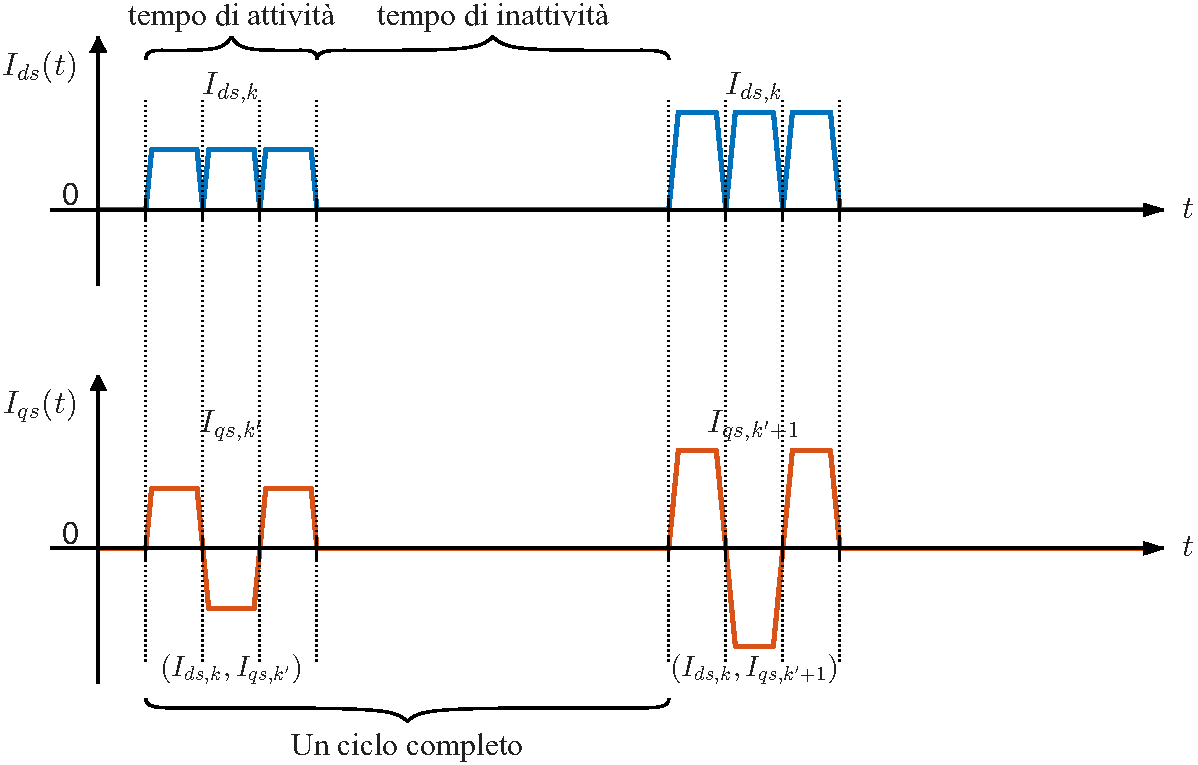
\includegraphics[height=7.5 cm]{immagini/grafici_matlab/Grafico_impulsi.pdf}
    \caption{Esempio della segquenza di impulsi $i_d$ e $i_q$.}
    \label{fig:Grafico_impulsi}
\end{figure}

\subsection{Stima del flusso in funzione della posizione elettrica}
\label{sec:stima_flusso}
Una volta raccolte le misure delle grandezze elettriche, si procede con la stima del flusso \cite{bojoi2024}.
Per comodità, si indicherà con $z_{x,k}^y$ un generico vettore di grandezze elettriche (tensione o corrente),$x$ si riferisce al sistema di riferimento $abc$, $\alpha\beta$ o $dq$, $y$ indica l'operazione $M_1$,$G$ o $M_2$ e $k$ l'indice del punto di misura nella griglia di corrente.
\begin{enumerate}
    \item Come primo passo, grandezze elettriche delle fasi di statore misurate $i^y_{abc,k}$, $v^y_{abc}$ devono essere riportate  secondo il sistema di riferimento $\alpha\beta$. Per far ciò i vettori di corrente e tensione vengono moltiplicati per la matrice di trasformazione.


\begin{equation}
\boldsymbol{z}_{\alpha\beta,k}^{y} = \frac{2}{3} \cdot 
\begin{bmatrix} 
1 & -\frac{1}{2} & -\frac{1}{2} \\ 
0 & -\frac{\sqrt{3}}{2} & \frac{\sqrt{3}}{2} 
\end{bmatrix} \cdot \boldsymbol{z}_{abc,k}^{y}
\label{eq:eq13}
\end{equation}

Basandosi sul (\ref{eq:eq13}), il flusso $\bf{\lambda}^y_{\alpha.\beta}$ può essere calcolato integrando la forza elettromotrice nel piano di riferimento $\alpha\beta$:

\begin{equation}
\boldsymbol{\lambda}_{\alpha\beta}^{y}(t) = \boldsymbol{\lambda}_{\alpha\beta}^{y}(t=0) + \int_{t_{0}}^{t_{0}+T} (\boldsymbol{v}_{\alpha\beta}^{y} - R_{s} \cdot \boldsymbol{i}_{\alpha\beta}^{y}) dt
\label{eq:integration_flux}
\end{equation}

dove $T$ corrisponde a una o più rivoluzioni meccaniche. La condizione iniziale del flusso può essere ottenuta tenendo conto che nel sistema $\alpha\beta$ in un periodo meccanico il flusso medio deve essere nullo:

\begin{equation}
\boldsymbol{\lambda}_{\alpha\beta}^{y}(t=0) = -mean \left( \int_{t_{0}}^{t_{0}+T} (v_{\alpha\beta}^{y} - R_{s} \cdot i_{\alpha\beta}^{y}) dt \right)
\end{equation}

\item \textbf{Interpolazione del flusso}: Dopo l'integrazione (\ref{eq:integration_flux}), le forme d'onda del flusso concatenato di M1,G e M2 sono determinate in funzione del tempo. A ogni istante temporale corrisponde un corrispettivo valore di posizione elettrica $\theta_e$. I vettori del flusso concatenato ottenuti per M1, G e M2 vengono ruotati dal sistema $\alpha\beta$ al sistema $dq$:

\begin{equation}
\boldsymbol{\lambda}_{dq,k}^y = 
\begin{bmatrix} 
\cos(\theta_e) & \sin(\theta_e) \\ 
-\sin(\theta_e) & \cos(\theta_e) 
\end{bmatrix} \cdot 
\boldsymbol{\lambda}_{\alpha\beta,k}^y \label{eq:matx_tr_dq}
\end{equation}

\item Calcolo delle mappe di flusso $dq\theta$: le stime di flusso durante le fasi M1, G e M2 sono ancora basate sull'integrazione (\ref{eq:integration_flux}), e così sensibili a errori dovuti al parametro resistivo. Per stimare le forme d'onda del flusso $\bm{\lambda}_{dq,k}^M(\bm{i}_{dq.k},\theta)$ e $\bm{\lambda}_{dq,k}^G(\bm{i}_{dq.k},\theta)$, includendo le armoniche spaziali e compensando la tensione resistiva, si applicano le seguenti espressioni:

\begin{subequations}
\label{eq:flussi_dq}
\begin{align}
    \lambda_d(\theta) &= \frac{\dfrac{\lambda_d^{M_1}(\theta_e) + \lambda_d^{M_2}(\theta_e)}{2} + \lambda_d^G(-\theta)}{2}  \\
    \lambda_q(\theta_e) &= \frac{\dfrac{\lambda_q^{M_1}(\theta_e) + \lambda_q^{M_2}(\theta_e)}{2} - \lambda_q^G(-\theta_e)}{2} \label{eq:estem_dq_l}
\end{align}
\end{subequations}

\end{enumerate}



\section{Stato dell'arte}
Esistono diversi metodi per stimare il flusso magnetico. Il modello magnetico del motore può essere estratto tramite delle simulazioni software ad elementi finiti (FEA).
Il metodo presentato in questa tesi permette di evitare l'utilizzo del software \cite{Zhao-Hong}.\\
Un problema che si riscontra nella stima del flusso è la variazione della resistenza a causa dell'aumento di temperatura.\\
Una possibile soluzione potrebbe essere quella di misurare la resistenza "on the fly", cioè prima della misurazione delle grandezze elettriche usate per stimare il flusso \cite{Gierczynski}. Tuttavia, questo metodo non permette di eliminare l'effetto dell'aumento di resistenza durante ciascuna degli stadi di misurazione (M1,G,M2).\\
Per quanto riguarda la misura di tensione, si può stimare la tensione a partire dal dutty-cycle, moltiplicando tale valore per la tensione di Bus. Dato che i tempi morti introducono un errore su questa stima, è necessario appliccare un algoritmo di compensazione il valore per ottenere il valore corretto \cite{Gierczynski}.\\

